\chapter{In Progress and Upcoming}
\section{Experiment 3: DenseCap}
The task on which a feature extractor is trained will effect the type of features it learns to identify. The goal of this experiment is to see if a model originally trained on a more language based task, such as captioning, identifies more relevant features for answering the questions. \\
The DenseCap model performs the 'dense captioning' task, in which the model identifies areas of interest in the image, and then provides a caption for each area\cite{densecap}. An example of the DenseCap output for an image from the scene dataset can be seen in Fig.~\ref{fig:example_densecap}. Some of the captions are a little bit weird, such as 'bathroom with walls and walls', but the model is identifying aspects such as color and material, which would be helpful in answering the types of questions being asked in the VQA portion. 

\begin{figure}[h]
     \centering
     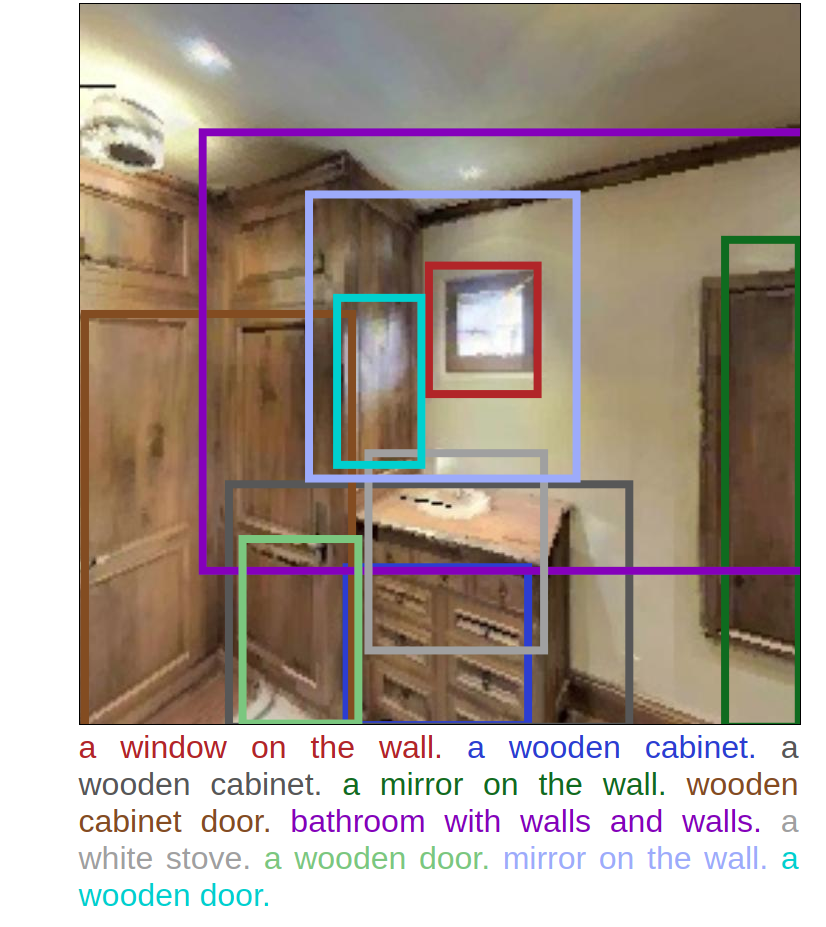
\includegraphics[width=.5\textwidth]{/home/yasmeen/Desktop/thesisproj/thesis/figure/example_densecap.png}
     \caption{DenseCap output for image from dataset}
     \label{fig:example_densecap}
\end{figure}


\subsection{Using DenseCap Features}
The first task, which is currently in progress, is to replace the original EQA CNN and use DenseCap as the feature extractor, as shown in Fig.~\ref{fig:densecap_feats}.

\begin{figure}[h]
     \centering
     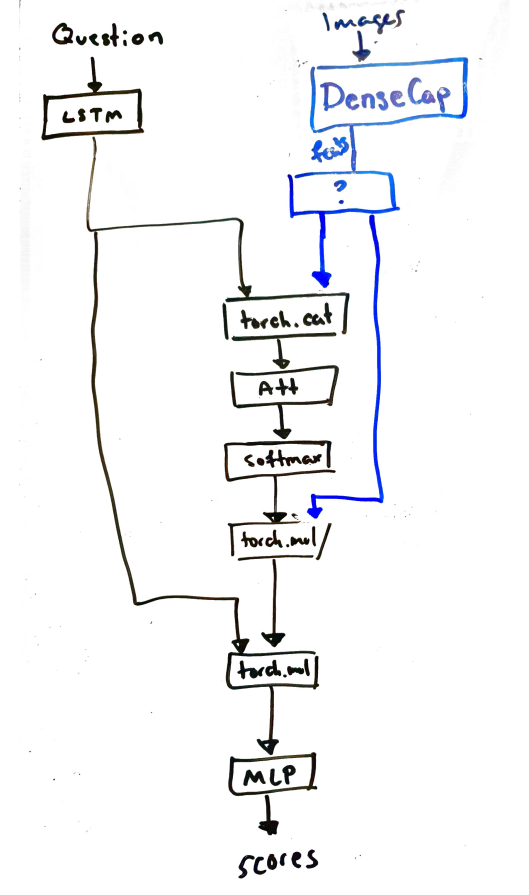
\includegraphics[width=.5\textwidth]{/home/yasmeen/Desktop/thesisproj/thesis/figure/densecapsketch.png}
     \caption{Model With Densecap}
     \label{fig:densecap_feats}
\end{figure}


\subsection{Using DenseCap Boxes}
Since DenseCap identifies areas of interest, these boxes can be used to give the model information about where objects are. I plan to give the model these boxes along with the features, as shown in Fig.~\ref{fig:densecap_boxes}. 

\begin{figure}[h]
     \centering
     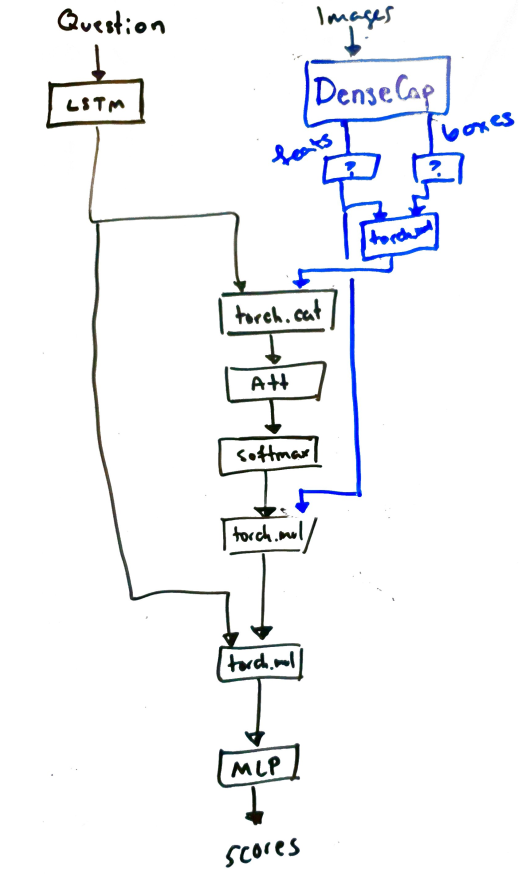
\includegraphics[width=.5\textwidth]{/home/yasmeen/Desktop/thesisproj/thesis/figure/densecapboxes.png}
     \caption{Model With Densecap Boxes}
     \label{fig:densecap_boxes}
\end{figure}
